%%%%%%%%%%%%%%%%%%%%%%%%%%%%%%%%%%%%%%%%%
% University/School Laboratory Report
% LaTeX Template
% Version 3.1 (25/3/14)
%
% This template has been downloaded from:
% http://www.LaTeXTemplates.com
%
% Original author:
% Linux and Unix Users Group at Virginia Tech Wiki 
% (https://vtluug.org/wiki/Example_LaTeX_chem_lab_report)
%
% License:
% CC BY-NC-SA 3.0 (http://creativecommons.org/licenses/by-nc-sa/3.0/)
%
%%%%%%%%%%%%%%%%%%%%%%%%%%%%%%%%%%%%%%%%%

%----------------------------------------------------------------------------------------
%	PACKAGES AND DOCUMENT CONFIGURATIONS
%----------------------------------------------------------------------------------------

\documentclass{article}

\usepackage[version=3]{mhchem} % Package for chemical equation typesetting
\usepackage{siunitx} % Provides the \SI{}{} and \si{} command for typesetting SI units
\usepackage{graphicx} % Required for the inclusion of images
\usepackage{natbib} % Required to change bibliography style to APA
\usepackage{amsmath} % Required for some math elements 
\usepackage{caption}
\usepackage{subcaption}
\usepackage{listings}
\usepackage{color}
 
\definecolor{codegreen}{rgb}{0,0.6,0}
\definecolor{codegray}{rgb}{0.5,0.5,0.5}
\definecolor{codepurple}{rgb}{0.58,0,0.82}
\definecolor{backcolour}{rgb}{0.95,0.95,0.92}
 
\lstdefinestyle{mystyle}{
    backgroundcolor=\color{backcolour},   
    commentstyle=\color{codegreen},
    keywordstyle=\color{codepurple},
    numberstyle=\tiny\color{codegray},
    stringstyle=\color{codepurple},
    basicstyle=\footnotesize,
    breakatwhitespace=false,         
    breaklines=true,                 
    captionpos=b,                    
    keepspaces=true,                 
    numbers=left,                    
    numbersep=5pt,                  
    showspaces=false,                
    showstringspaces=false,
    showtabs=false,                  
    tabsize=2
}
\lstset{style=mystyle}

\setlength\parindent{0pt} % Removes all indentation from paragraphs

\renewcommand{\labelenumi}{\alph{enumi}.} % Make numbering in the enumerate environment by letter rather than number (e.g. section 6)

\newcommand\tab[1][0.5cm]{\hspace*{#1}}

%\usepackage{times} % Uncomment to use the Times New Roman font

%----------------------------------------------------------------------------------------
%	DOCUMENT INFORMATION
%----------------------------------------------------------------------------------------

\title{COMP 429/529: Project 1} % Title

\author{Berkay \textsc{Barlas}} % Author name

\date{\today} % Date for the report

\begin{document}

\maketitle % Insert the title, author and date

\begin{center}
\begin{tabular}{l r}
Date Performed: & March 17, 2019 \\ % Date the experiment was performed
Instructor: & Didem Unat % Instructor/supervisor
\end{tabular}
\end{center}

% If you wish to include an abstract, uncomment the lines below
% \begin{abstract}
% Abstract text
% \end{abstract}

%----------------------------------------------------------------------------------------
%	SECTION 1
%----------------------------------------------------------------------------------------

\tab In this assignment I developed my parallel implementations 
on top of given serial version for two different applications;
an image blurring algorithm and sudoku solver using OpenMP. 
\newline While the first application in data parallelism, 
the second application in task parallelism. 
\newline
\newline
In this assignment I have completed
\begin{itemize}
    \item Parallel Version of Image Blurring
    \item Performance Study for Part I
    \item Parallel Version of Sudoku Part A, Part B, Part C
    \item Performance Study for Part II 
\end{itemize}


\section{Part I: Image Blurring}


\tab In the first part of this assignment I implemented 
a parallel version of a simple image blurring algorithm with
OpenMP which takes an input image and outputs a blurred image.
\\
\tab I used \#pragma omp for collapse() in getGaussian(), loadImage(), saveImage(), applyFilter(), averageRGB() 
methods since all of have nested for loops that can be parallelized. The biggest nested for loop is in applyFilter() 
and it can be parallelizable as below. collapse(5) can not be used because last two for loops depends on previous loops.
\begin{lstlisting}[language=C]
    #pragma omp parallel for collapse(3)
    for (d=0 ; d<3 ; d++) {
     for (i=0 ; i<newImageHeight ; i++) {
      for (j=0 ; j<newImageWidth ; j++) {
       for (h=0 ; h<filterHeight ; h++) {
        for (w=0 ; w<filterWidth ; w++) {
            newImage[d][i][j] += filter[h][w]*image[d][h+i][w+j];
    }}}}}
\end{lstlisting}

\newpage
\subsection{Stability Test}

\begin{description}
    \item[Serial version execution time: ] \hfill \\ 
    Coffee Image: 13.64\\
    Strawberry Image: 27.56\\
    \item[Paralel version with single thread execution time: ] \hfill \\
    Coffee Image: 30.88\\
    Strawberry Image: 55.93\\
    \item[Which thread number gives the best performance?] \hfill \\
    32 thread count gives the best performance for both blurring applications.
    \\
    The reason of serial version performs better than parallel version with 1 thread is Parallization overhead.
    The difference between them caused by the execution time of parallization.
\end{description}

\textbf{Results}

\begin{figure}[!htb]
    \centering
    \begin{subfigure}{.45\textwidth}
        \centering
        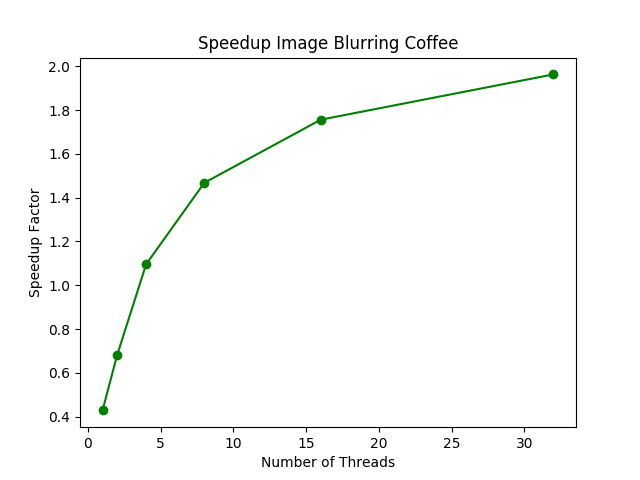
\includegraphics[width=1\linewidth]{./img/speedup_part_1_A.png}
        \caption{Speedup results for the blurring on coffee image.}
    \end{subfigure} 
    \begin{subfigure}{.45\textwidth}
        \centering
        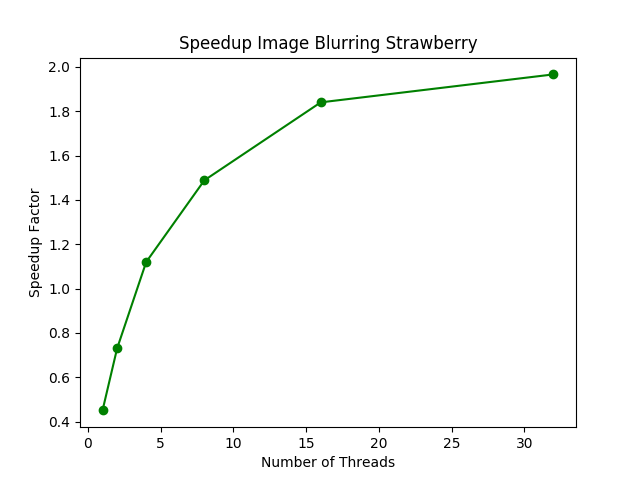
\includegraphics[width=1\linewidth]{./img/speedup_part_1_A_strawberry.png}
        \caption{Speedup results for the blurring on strawberry image.}
    \end{subfigure}
    \caption{Speedup figures for image blurring application}
\end{figure}   

\textbf{Explanation of Speedup Curve}
\\
\tab Due to parallization overhead a speedup with value bigger than 1 is observed after 4 threads for both applications. \\
\tab Even though, a linear/perfect speedup is not expected the results are actually worse than what is expected.
Even the parallel version with 32 thread on 32 core cluster gives only around 2x speedup.\\
One of reasons of that is intel compiler optimizations in serial version which is already very fast.\\

\newpage

\subsection{Thread Binding Test}
\tab In the compact mapping, multiple threads are mapped as close as possible to each other, 
while in the scatter mapping, the threads are distributed as evenly as possible across all cores. 

\begin{description}
    \item[Different mapping strategies; Compact and Scatter]
\end{description}
\textbf{Results}
 \begin{figure}[!htb]
    \centering
    \begin{subfigure}{.45\textwidth}
        \centering
        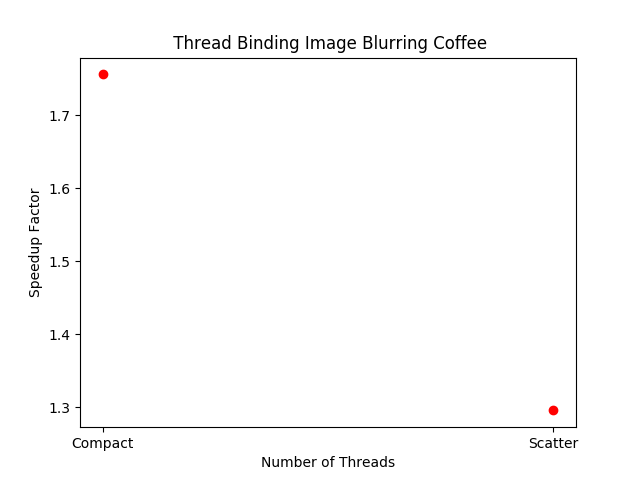
\includegraphics[width=1\linewidth]{./img/binding_part_1_B_coffee.png}
        \caption{Results for the blurring on coffee image.}
    \end{subfigure} 
    \begin{subfigure}{.45\textwidth}
        \centering
        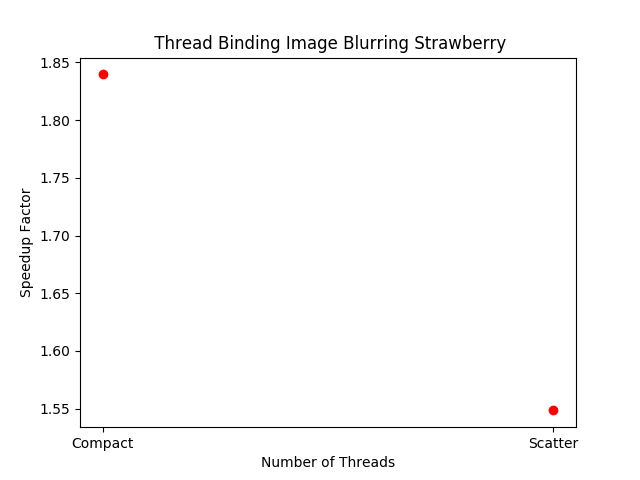
\includegraphics[width=1\linewidth]{./img/binding_part_1_B_strawberry.png}
        \caption{Results for the blurring on strawberry image.}
    \end{subfigure}
    \caption{Speedup figures for image blurring application}
\end{figure}

\textbf{Which Mapping Gives Better Performance, Why?}\\
\\ \tab Compact gives better performance for both images because 
when neighbouring threads are accessing the same(Temporal Locality) or nearby data(Spatial Locality);
the data which is brought into the cache by one thread can be used 
by the other, avoiding a costly memory access.
If the tasks were longer scatter could perform better. 

%----------------------------------------------------------------------------------------
%	SECTION 2
%----------------------------------------------------------------------------------------
\newpage

\section{PART II: Parallel Sudoku Solver}
\tab In the second part of this assignment, I parallelized a serial sudoku solver with OpenMP
which takes a sudoku problem as an input and finds all possible solutions from it 
using a brute force search for searching by all possible solutions to the problem. 
\\ \textbf{Part A}
\\ \tab In this Part, I defined parallel section while calling solveSudoku() method. I used \#pragma omp task in different places inside solveSudoku() method, after several run and experiments using I selected the one that gives best performance.
\begin{lstlisting}[language=C]
if(matrix[row][col] != EMPTY) {
//#pragma omp task firstprivate(col, row)
    if (solveSudoku(row, col+1, matrix, box_sz, grid_sz)) { 
            printMatrix(matrix, box_sz); 
    }
} else {
int num;
  for (num = 1; num <= box_sz; num++) 
  { 					
   if (canBeFilled(matrix, row, col, num, box_sz, grid_sz)) 
   {  
    #pragma omp task firstprivate(num, col, row)
    {
     int tempMatrix[MAX_SIZE][MAX_SIZE];
     int i;
     int j;
     for(i=0; i<box_sz; i++) {
         for( j=0; j<box_sz; j++){
             tempMatrix[i][j] = matrix[i][j];
         }
     }
     tempMatrix[row][col] = num; 				
     if (solveSudoku(row, col+1, tempMatrix, box_sz, grid_sz)) 
         printMatrix(tempMatrix, box_sz);
    }					
   }
  }
}		
\end{lstlisting}
\newpage

\textbf{Part B}
\\ \tab In this Part, I changed funtion signature to pass the task depth. Every time, a new task is created 
the depth value is incereased by 1 and passed to recursive method as parameter.
\\ \tab To find a good cutoff value I run the program with different cutoff parameters. Overall cutoff value 30 gived the best result.
\begin{lstlisting}[language=C]
if (canBeFilled(matrix, row, col, num, box_sz, grid_sz)) 
{  
 #pragma omp task firstprivate(num, col, row, depth) if (depth < MAX_DEPTH)
 {
  depth++;
  int tempMatrix[MAX_SIZE][MAX_SIZE];
  int i;
  int j;
  for(i=0; i<box_sz; i++) {
      for( j=0; j<box_sz; j++){
          tempMatrix[i][j] = matrix[i][j];
      }
  }
  tempMatrix[row][col] = num; 				
  if (solveSudoku(row, col+1, tempMatrix, box_sz, grid_sz, depth)) 
      printMatrix(tempMatrix, box_sz);
 }					
}
\end{lstlisting}

\textbf{Part C}
\\ \tab In this Part, I created a shared variable found and passed it as 
parameter to solveSudoku function which stops priting solution and creation of new tasks.  
\begin{lstlisting}[language=C]
#pragma omp parallel shared(found)
{
	#pragma omp single 
	{
	solveSudoku(0, 0, matrix, box_sz, grid_sz, &found);
	}
}
\end{lstlisting}
I also used \#pragma omp critical when I changing value of found.
\begin{lstlisting}[language=C]
    ...
    #pragma omp critical
        *found = 1; 
    ...
\end{lstlisting}
\newpage

\subsection{Scalability Test}
\subsubsection{Part A}
\begin{description}
\item[Serial version execution time: ] 48.10
\item[Paralel version with single thread execution time: ] 78.69
\item[Which thread number gives the best performance?]\hfill \\
32 thread count gives the best performance.
\end{description} 

\textbf{Results}
 \begin{figure}[!htb]
    \centering
        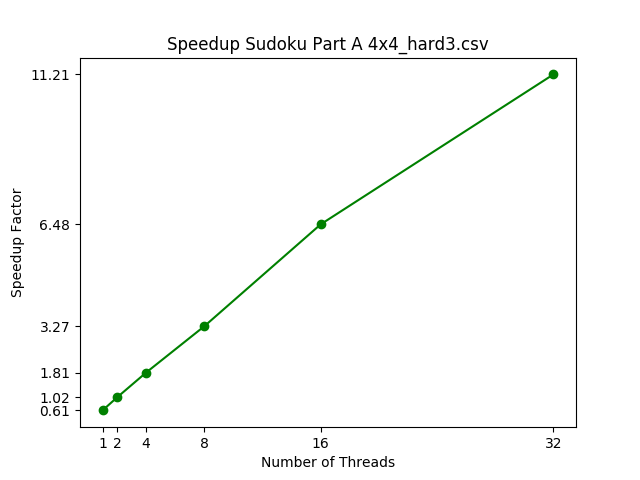
\includegraphics[width=0.8\linewidth]{./img/speedup_part_2_A.png}
        \caption{\small Results for the Sudoku 4x4hard3 using algorithm in.}
\end{figure}                

\textbf{Explanation of Speedup Curve}\\
\tab Due to parallization overhead a speedup with value bigger than 1 is observed after 2 threads. \\
\tab The task Parallization of serial version results in the creation of different task
causes to a great overhead.
Therefore, the speedup results are lower than expected. Even with 32 thread speedup is just around 11.
\newpage

\subsubsection{Part B}

\begin{description}
\item[Serial version execution time: ] 48.10
\item[Paralel version with single thread execution time: ] 74.50
\item[Which thread number gives the best performance?]\hfill \\
32 thread count gives the best performance.

\end{description} 
\begin{figure}[!htb]
        \centering
        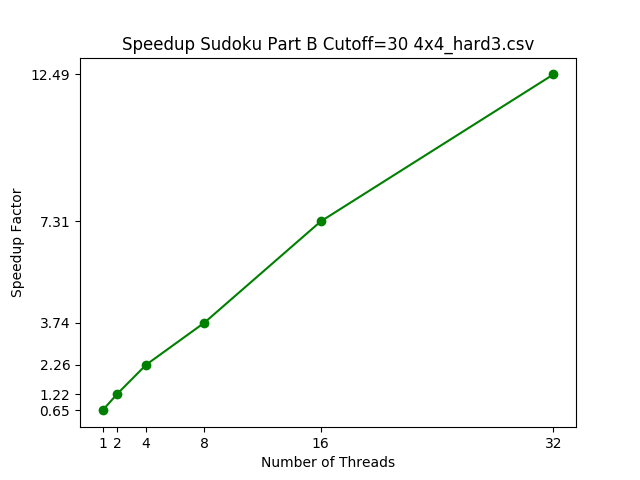
\includegraphics[width=1\linewidth]{./img/speedup_part_2_B.png}
        \caption{Results for the blurring on strawberry image.}
\end{figure}
\textbf{Explanation of Speedup Curve}\\
\tab Due to parallization overhead a speedup with value bigger than 1 is observed after 2 threads. \\
\tab In order to improve the performance of the previous parallel version, a cutoff parameter 
to limit the number of parallel tasks is needed.\\
\tab I defined a variable called depth and passed it as parameter to recursive method  
to prevent task creation after certain depth in the call-path tree. 
After that depth switch to the serial execution and do not generate more tasks.
To determine that cut off parameter, I executed parallel program with several
different values.\\
\tab The speedup curve is linear which is expected.  

\newpage

\subsubsection{Part C}
\begin{description}
\item[Serial version execution time: ] 0.33
\item[Paralel version with single thread execution time: ] 0.57
\item[Which thread number gives the best performance?]\hfill \\
32 thread count gives the best performance.
\end{description} 

\begin{figure}[!htb]
        \centering
        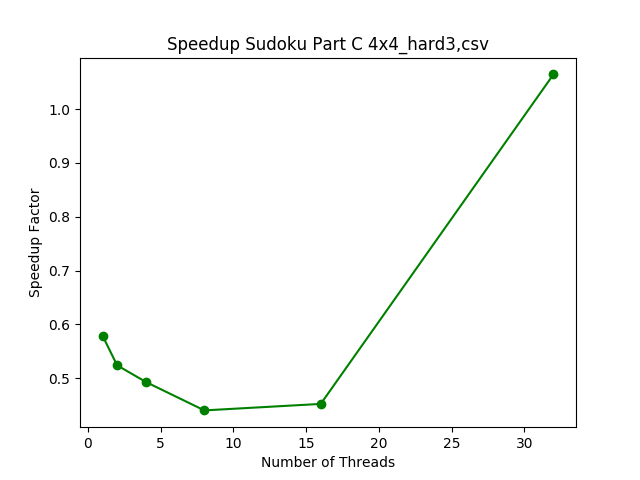
\includegraphics[width=1\linewidth]{./img/speedup_part_2_C.png}
        \caption{Results for the blurring on strawberry image.}
\end{figure}
\textbf{Explanation of Speedup Curve}
\\
\tab Stopping the execution after finding a solution is very easy for 
serial version which can be done by returning a different value 
inside of for loops when a solution is found.
In order to guraantee single solution in parallel version a shared variable 'found'
which will stop further task creation and execution can be defined.
In this application, parallized application results are really poor 
because a solution might be found by one of the tasks but other tasks that are created previously
will continue execution and this creates a great overhead compared to serial version.
\\ \tab Also, from 1 thread to 16 thread, increasing the number of threads decreases to speedup. 
This is most likely to be caused by increased number of total task created and needs to be executed, even though, 
one of the tasks already find a solution.
\newpage

\subsection{Thread Binding Test}
\subsubsection{Part A}
\begin{description}
    \item[Different mapping strategies; Compact and Scatter]
\end{description}
\begin{figure}[!htb]
    \centering
    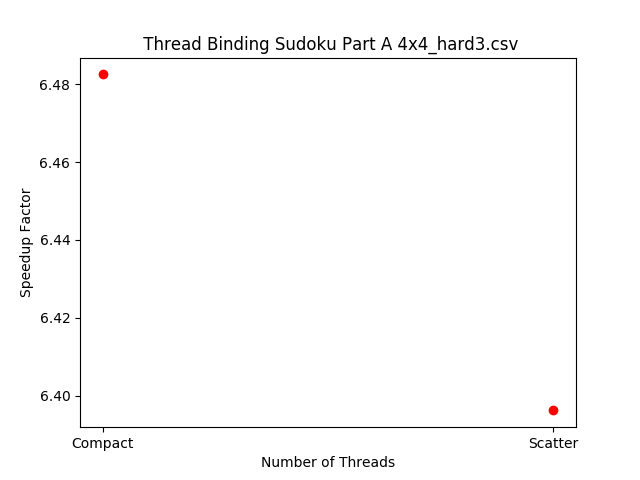
\includegraphics[width=1\linewidth]{./img/binding_part_2_A.png}
    \caption{Results for the blurring on strawberry image.}
\end{figure}
\textbf{Which Mapping Gives Better Performance, Why?}\\
\\ \tab Compact gives better performance for both images because 
when neighbouring threads are accessing the same(Temporal Locality) or nearby data(Spatial Locality);
the data which is brought into the cache by one thread can be used 
by the other, avoiding a costly memory access.
If the tasks were longer scatter could perform better. 


\newpage

\subsubsection{Part B}
\begin{description}
    \item[Different mapping strategies; Compact and Scatter]
\end{description}
\begin{figure}[!htb]
    \centering
    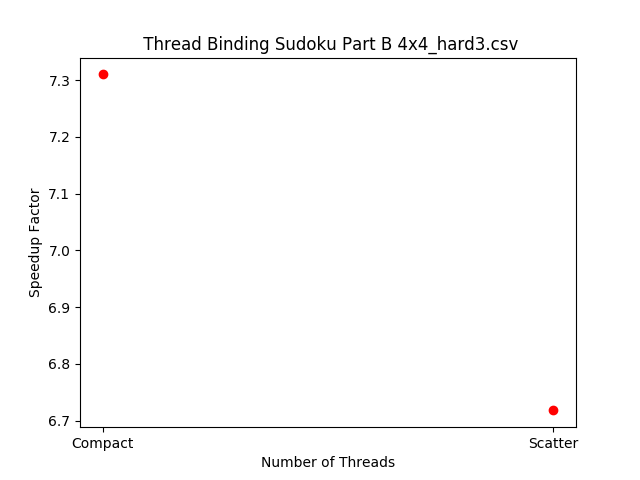
\includegraphics[width=1\linewidth]{./img/binding_part_2_B.png}
    \caption{Results for the blurring on strawberry image.}
\end{figure}
\textbf{Which Mapping Gives Better Performance, Why?}\\
\\ \tab Compact gives better performance for both images because 
when neighbouring threads are accessing the same(Temporal Locality) or nearby data(Spatial Locality);
the data which is brought into the cache by one thread can be used 
by the other, avoiding a costly memory access.
If the tasks were longer scatter could perform better. 

\newpage

\subsubsection{Part C}
\begin{description}
    \item[Different mapping strategies; Compact and Scatter]
\end{description}
\begin{figure}[!htb]
    \centering
    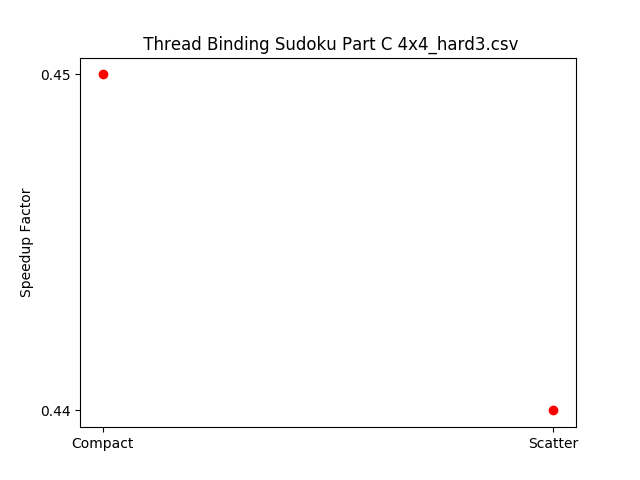
\includegraphics[width=1\linewidth]{./img/binding_part_2_C.png}
    \caption{Results for the blurring on strawberry image.}
\end{figure}
\textbf{Which Mapping Gives Better Performance, Why?}\\
\\ \tab Compact gives better performance for both images because 
when neighbouring threads are accessing the same(Temporal Locality) or nearby data(Spatial Locality);
the data which is brought into the cache by one thread can be used 
by the other, avoiding a costly memory access.
If the tasks were longer scatter could perform better. 

\newpage

\subsection{Tests on Sudoku Problems of Different Grids}
\begin{description}
\item[Part-B]
\end{description} 
\begin{figure}[!htb]
    \centering
    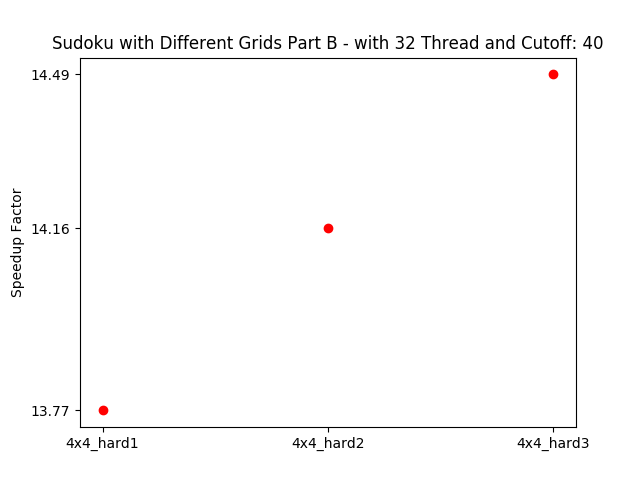
\includegraphics[width=1\linewidth]{./img/grids_part_2_B.png}
    \caption{Results for the 32 Thread Parallel Sudoku solver in Part B with different sizes and difficulties.}
\end{figure}
\tab When the difficulties of sudoku problem increases parallized algorithm in Part B performs better 
over serial serial version. Effectiveness of parallization increases beacuse when the task difficulty
increased the execution time ratio of parallelizable partion over non-parallelizable partion increases. 

%----------------------------------------------------------------------------------------
%	SECTION 6
%----------------------------------------------------------------------------------------

\section{Formulas Used}

\begin{enumerate}
\begin{item}
    \emph{Speedup} 
    \begin{equation*}
    Speedup  = \frac{\mathrm{T1}}{\mathrm{Tp}}
    %\begin{center}\ce{}\end{center}
    \end{equation*}
\end{item}
\begin{item}
    \emph{Amdahl's Law} 
    \begin{equation*}
    Tp \geq Wserial + \frac{\mathrm{Wparallel}}{\mathrm{P}}
    %\begin{center}\ce{}\end{center}
    \end{equation*}
\end{item}
\end{enumerate}




\end{document}